\begin{figure}[htbp]
		\centering
		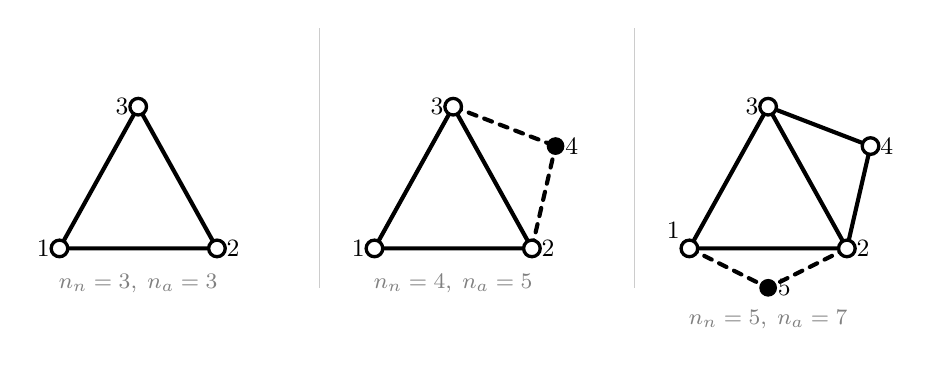
\begin{tikzpicture}[
			scale=1.0,
			asta/.style={line width=1.5pt, line cap=round,
				line join=round, black},
			nuova/.style={line width=1.5pt, line cap=round,
				line join=round, black, dashed},
			nodo/.style={circle, fill=white, draw=black,
				inner sep=0pt, minimum size=6pt,
				line width=1.2pt},
			nuovonodo/.style={circle, fill=black,
				draw=black, inner sep=0pt,
				minimum size=6pt},
			]
			\draw[very thin, gray!40](3.8,-0.5)--(3.8,2.8);
			\draw[very thin, gray!40](7.8,-0.5)--(7.8,2.8);
			
			\coordinate (A0) at (0.5, 0);
			\coordinate (B0) at (2.5, 0);
			\coordinate (C0) at (1.5, 1.8);
			\draw[asta](A0)--(B0)--(C0)--(A0);
			\node[nodo] at (A0){}; \node[nodo] at (B0){};
			\node[nodo] at (C0){};
			\node[left, font=\small] at (A0){$1$};
			\node[right,font=\small] at (B0){$2$};
			\node[left, font=\small] at (C0){$3$};
			\node[font=\footnotesize,gray] at (1.5,-0.45)
			{$n_n=3,\;n_a=3$};
			
			\coordinate (A1) at (4.5, 0);
			\coordinate (B1) at (6.5, 0);
			\coordinate (C1) at (5.5, 1.8);
			\coordinate (D1) at (6.8, 1.3);
			\draw[asta](A1)--(B1)--(C1)--(A1);
			\draw[nuova](B1)--(D1);
			\draw[nuova](C1)--(D1);
			\node[nodo] at (A1){}; \node[nodo] at (B1){};
			\node[nodo] at (C1){}; \node[nuovonodo] at (D1){};
			\node[left, font=\small] at (A1){$1$};
			\node[right,font=\small] at (B1){$2$};
			\node[left, font=\small] at (C1){$3$};
			\node[right,font=\small] at (D1){$4$};
			\node[font=\footnotesize,gray] at (5.5,-0.45)
			{$n_n=4,\;n_a=5$};
			
			\coordinate (A2) at (8.5,  0);
			\coordinate (B2) at (10.5, 0);
			\coordinate (C2) at (9.5,  1.8);
			\coordinate (D2) at (10.8, 1.3);
			\coordinate (E2) at (9.5, -0.5);
			\draw[asta](A2)--(B2)--(C2)--(A2);
			\draw[asta](B2)--(D2);
			\draw[asta](C2)--(D2);
			\draw[nuova](A2)--(E2);
			\draw[nuova](B2)--(E2);
			\node[nodo] at (A2){}; \node[nodo] at (B2){};
			\node[nodo] at (C2){}; \node[nodo] at (D2){};
			\node[nuovonodo] at (E2){};
			\node[above left,font=\small] at (A2){$1$};
			\node[right,     font=\small] at (B2){$2$};
			\node[left,      font=\small] at (C2){$3$};
			\node[right,     font=\small] at (D2){$4$};
			\node[right,     font=\small] at (E2){$5$};
			\node[font=\footnotesize,gray] at (9.5,-0.90)
			{$n_n=5,\;n_a=7$};
		\end{tikzpicture}
		\caption{Costruzione gerarchica di una travatura
			reticolare internamente isostatica.
			A sinistra: triangolo base ($n_n = 3$,
			$n_a = 3$). Al centro: aggiunta del primo
			nodo ($n_n = 4$, $n_a = 5$). A destra:
			aggiunta del secondo nodo ($n_n = 5$,
			$n_a = 7$). In ciascun passo le due aste
			nuove sono tratteggiate e il nuovo nodo è
			indicato con un cerchio pieno.}
		\label{fig:reticolare_gerarchia}
	\end{figure}
